\documentclass[aspectratio=169]{../latex_main/tntbeamer}  % you can pass all options of the beamer class, e.g., 'handout' or 'aspectratio=43'
\usepackage{dsfont}
\usepackage{bm}
\usepackage[english]{babel}
\usepackage[T1]{fontenc}
%\usepackage[utf8]{inputenc}
\usepackage{graphicx}
\graphicspath{ {./figures/} }
\usepackage{algorithm}
\usepackage[ruled,vlined,algo2e,linesnumbered]{algorithm2e}
\usepackage{hyperref}
\usepackage{booktabs}
\usepackage{mathtools}

\usepackage{amsmath,amssymb}

\DeclareMathOperator*{\argmax}{arg\,max}
\DeclareMathOperator*{\argmin}{arg\,min}

\usepackage{amsbsy}
\newcommand{\vect}[1]{\bm{#1}}
%\newcommand{\vect}[1]{\boldsymbol{#1}}

\usepackage{pgfplots}
\pgfplotsset{compat=1.16}
\usepackage{tikz}
\usetikzlibrary{trees} 
\usetikzlibrary{shapes.geometric}
\usetikzlibrary{positioning,shapes,shadows,arrows,calc,mindmap}
\usetikzlibrary{positioning,fadings,through}
\usetikzlibrary{decorations.pathreplacing}
\usetikzlibrary{intersections}
\pgfdeclarelayer{background}
\pgfdeclarelayer{foreground}
\pgfsetlayers{background,main,foreground}
\tikzstyle{activity}=[rectangle, draw=black, rounded corners, text centered, text width=8em]
\tikzstyle{data}=[rectangle, draw=black, text centered, text width=8em]
\tikzstyle{myarrow}=[->, thick, draw=black]

% Define the layers to draw the diagram
\pgfdeclarelayer{background}
\pgfdeclarelayer{foreground}
\pgfsetlayers{background,main,foreground}

% Requires XeLaTeX or LuaLaTeX
%\usepackage{unicode-math}

\usepackage{fontspec}
%\setsansfont{Arial}
\setsansfont{RotisSansSerifStd}[ 
Path=../latex_main/fonts/,
Extension = .otf,
UprightFont = *-Regular,  % or *-Light
BoldFont = *-ExtraBold,  % or *-Bold
ItalicFont = *-Italic
]
\setmonofont{Cascadia Mono}[
Scale=0.8
]

% scale factor adapted; mathrm font added (Benjamin Spitschan @TNT, 2021-06-01)
%\setmathfont[Scale=1.05]{Libertinus Math}
%\setmathrm[Scale=1.05]{Libertinus Math}

% other available math fonts are (not exhaustive)
% Latin Modern Math
% XITS Math
% Libertinus Math
% Asana Math
% Fira Math
% TeX Gyre Pagella Math
% TeX Gyre Bonum Math
% TeX Gyre Schola Math
% TeX Gyre Termes Math

% Literature References
\newcommand{\lit}[2]{\href{#2}{\footnotesize\color{black!60}[#1]}}

%%% Beamer Customization
%----------------------------------------------------------------------
% (Don't) Show sections in frame header. Options: 'sections', 'sections light', empty
\setbeamertemplate{headline}{empty}

% Add header logo for normal frames
\setheaderimage{
	% 
\includegraphics[height=\logoheight]{figures/TNT_darkv4.pdf}
	
\includegraphics[height=\logoheight]{../latex_main/figures/luh_logo_rgb_0_80_155.pdf}
	% 
\includegraphics[height=\logoheight]{figures/logo_tntluh.pdf}
}

% Header logo for title page
\settitleheaderimage{
	% 
\includegraphics[height=\logoheight]{figures/TNT_darkv4.pdf}
	
\includegraphics[height=\logoheight]{../latex_main/figures/luh_logo_rgb_0_80_155.pdf}
	% 
\includegraphics[height=\logoheight]{figures/logo_tntluh.pdf}
}

% Title page: tntdefault 
\setbeamertemplate{title page}[tntdefault]  % or luhstyle
% Add optional title image here
%\addtitlepageimagedefault{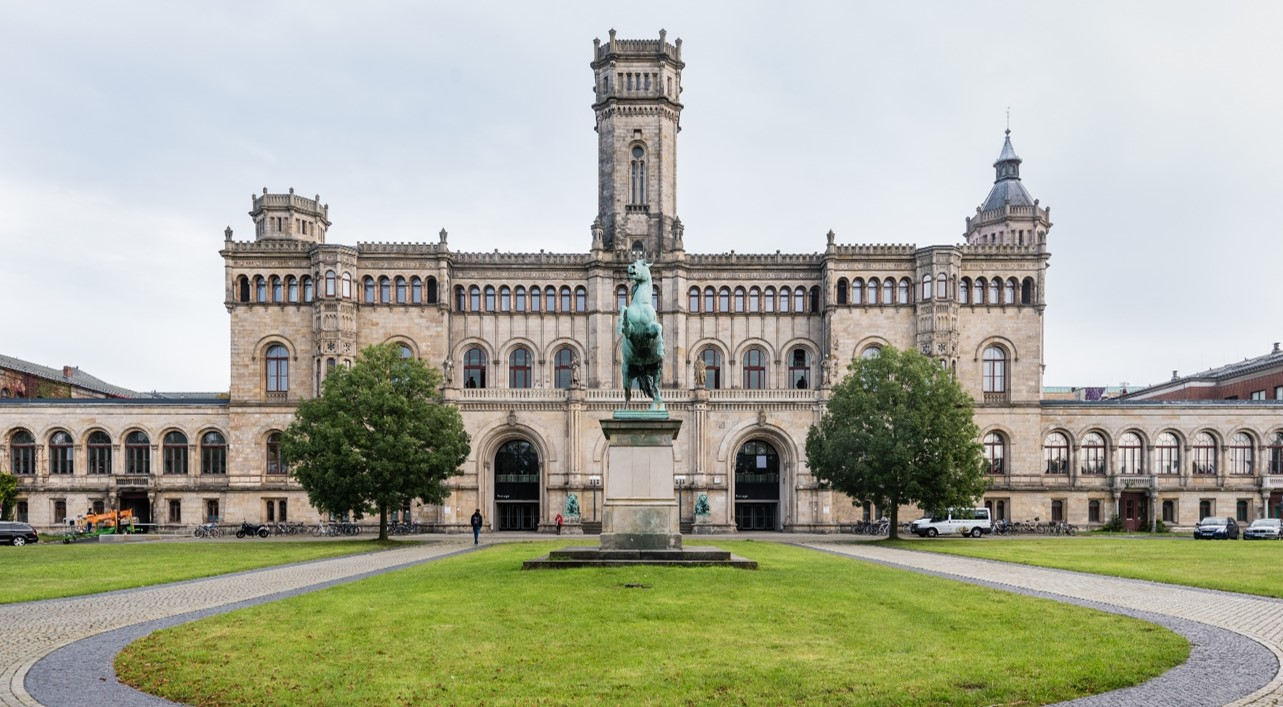
\includegraphics[width=0.65\textwidth]{figures/luh_default_presentation_title_image.jpg}}

% Title page: luhstyle
% \setbeamertemplate{title page}[luhstyle]
% % Add optional title image here
% \addtitlepageimage{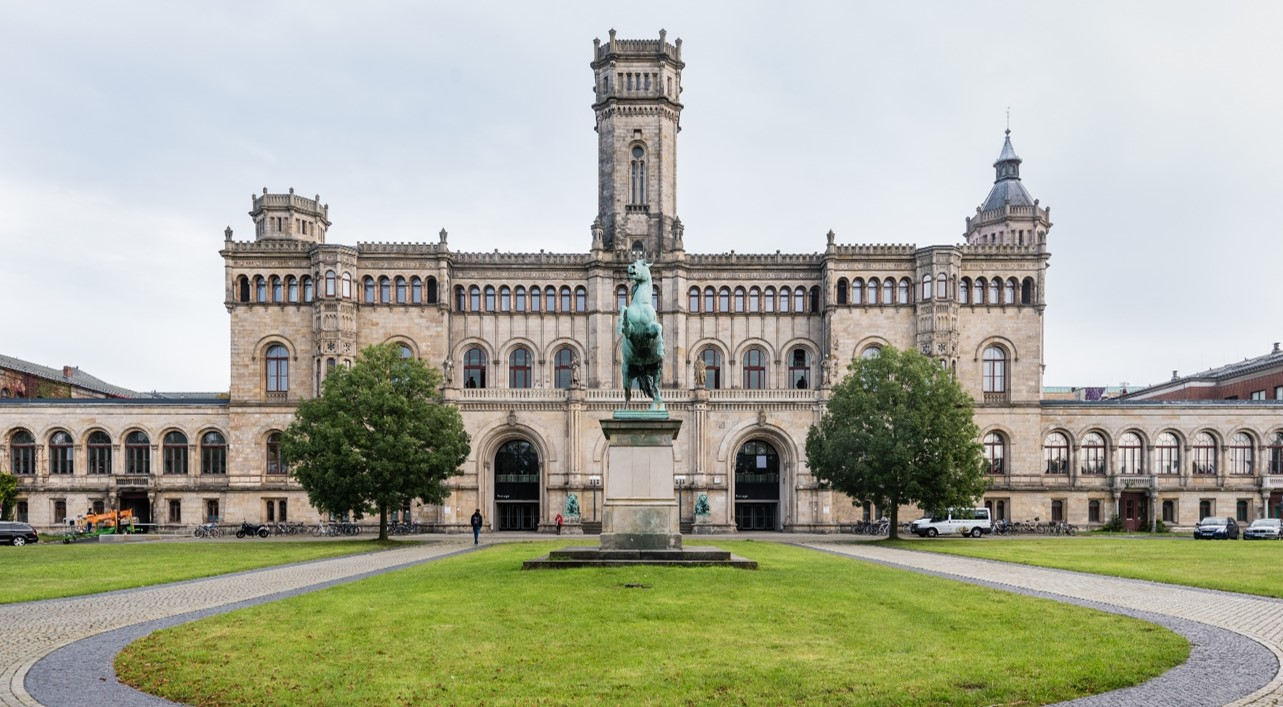
\includegraphics[width=0.75\textwidth]{figures/luh_default_presentation_title_image.jpg}}

\author[Abedjan \& Lindauer]{Ziawasch Abedjan \& Marius Lindauer\\[1em]
	
\includegraphics[height=\logoheight]{../latex_main/figures/luh_logo_rgb_0_80_155.pdf}\qquad
	
\includegraphics[height=\logoheight]{../latex_main/figures/DBIS_Kurzlogo.png}\qquad

\includegraphics[height=\logoheight]{../latex_main/figures/TNT_darkv4}\qquad

\includegraphics[height=\logoheight]{../latex_main/figures/L3S.jpg}	}
\date{Summer Term 2022; \hspace{0.5em} {
\includegraphics[height=1.5em]{../latex_main/figures/Cc-by-nc-sa_icon.svg.png}}; based on \href{https://ds100.org/fa21/}{[DS100]}
}


%%% Custom Packages
%----------------------------------------------------------------------
% Create dummy content
\usepackage{blindtext}

% Adds a frame with the current page layout. Just call \layout inside of a frame.
\usepackage{layout}


%%% Macros
%\renewcommand{\vec}[1]{\mathbf{#1}}
% \usepackage{bm}
%\let\vecb\bm

\title[Regression]{DS: Learning}
\subtitle{Supervised Learning: Regression}

\graphicspath{ {./figure/} }
%\institute{}


\begin{document}
	
    \maketitle
    
    \begin{frame}[c]{What is Regression?}
        \begin{itemize}
            \item Supervised learning considers learning $f: x \mapsto y$ from training data $\mathcal{D}= \{(x_i,y_i)\}_{i}$ 
            \item If $y$ is a continuous variable we consider it as a regression problem
            \item (Time series prediction can be seen a special case of regression problems)
        \end{itemize} 

        \centering
        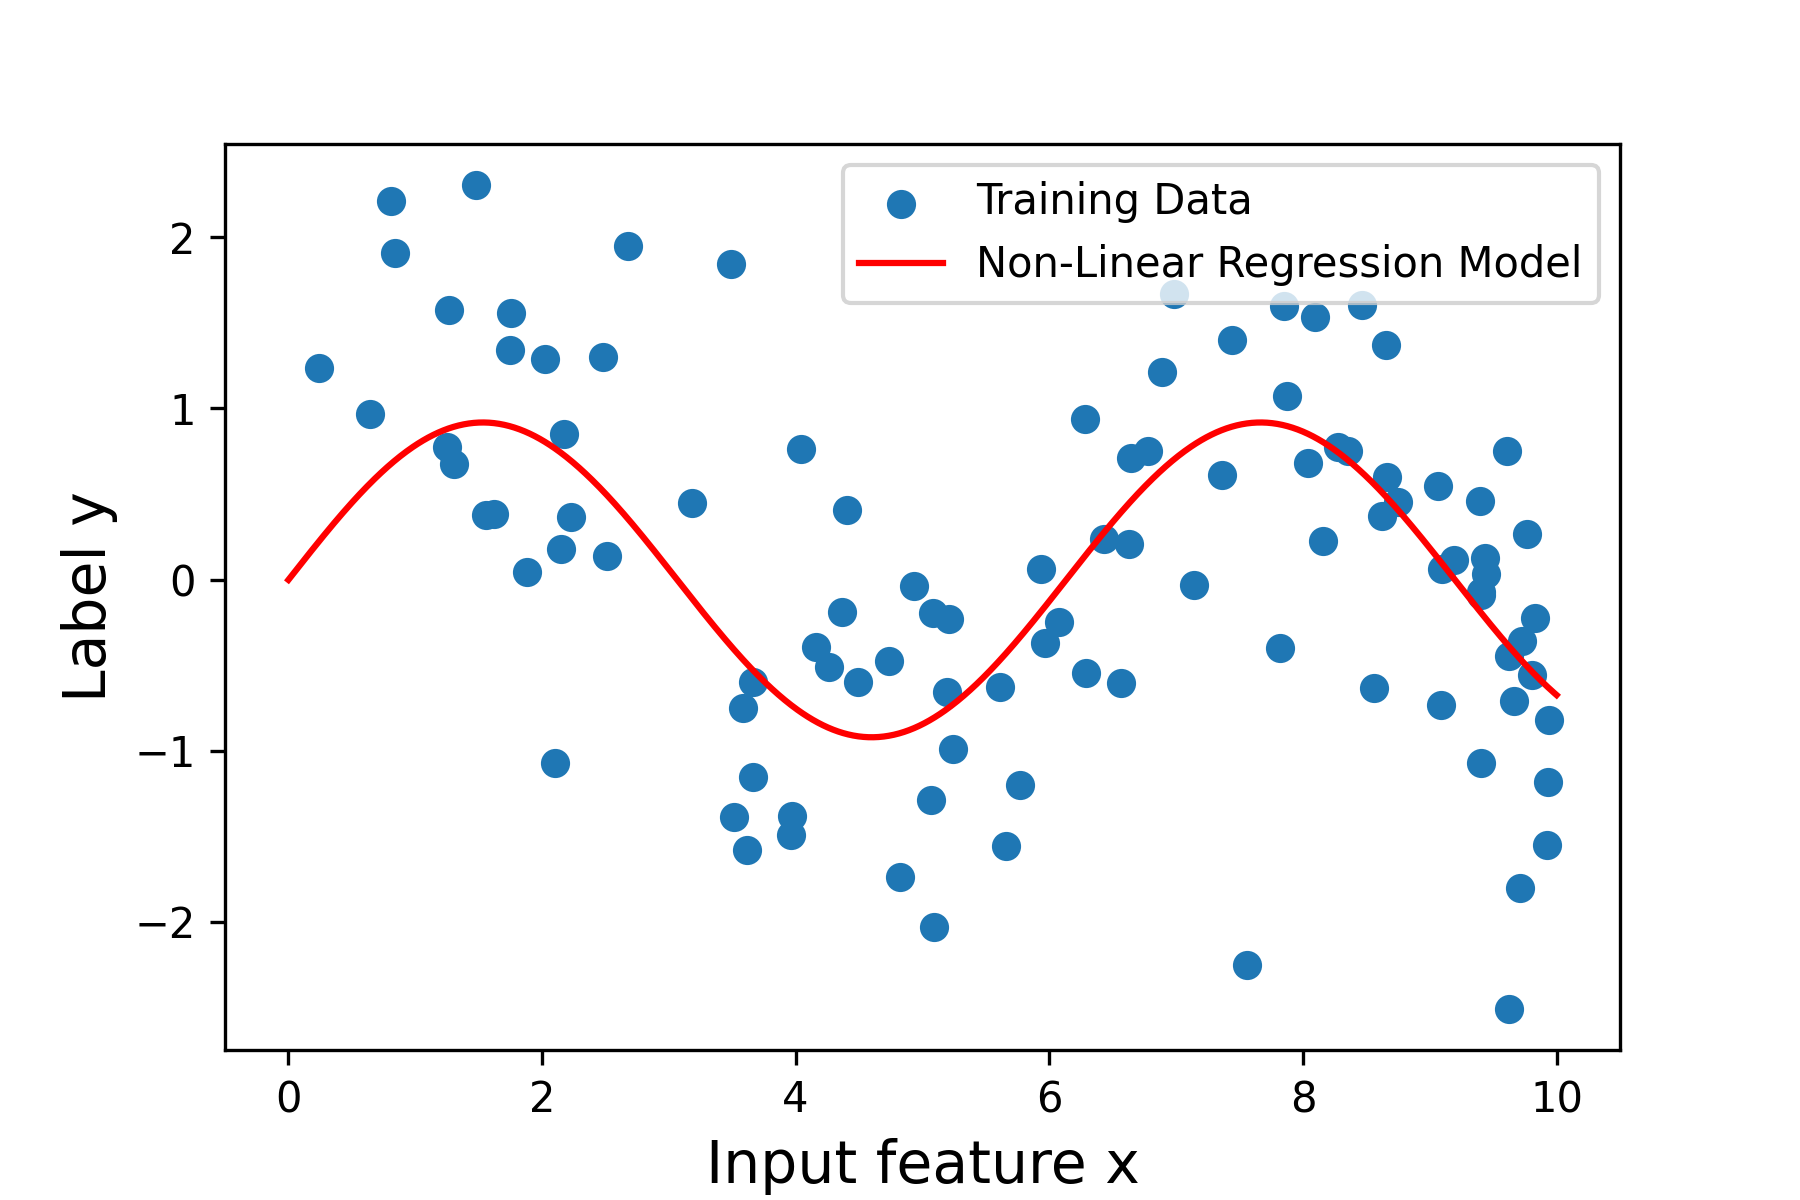
\includegraphics[width=0.5\textwidth]{figure/nonlinear_regression}

        % import numpy as np
        % import matplotlib.pyplot as plt
        % from sklearn.mixture import GaussianMixture
        
        % # generate some data points with outliers
        % np.random.seed(42)
        % X_train = np.concatenate([np.random.normal(size=(200, 2)), np.random.normal(5, size=(10, 2))])
        
        % # fit a Gaussian mixture model
        % gmm = GaussianMixture(n_components=2)
        % gmm.fit(X_train)
        
        % # create a grid of points to evaluate the model
        % xx, yy = np.meshgrid(np.linspace(-7, 7, 100), np.linspace(-7, 7, 100))
        % Z = -gmm.score_samples(np.c_[xx.ravel(), yy.ravel()])
        % Z = Z.reshape(xx.shape)
        
        % # plot the data and the contour lines of the model
        % plt.figure(figsize=(8, 6), dpi=300)
        % plt.scatter(X_train[:, 0], X_train[:, 1], c='black')
        % plt.contour(xx, yy, Z, levels=[3], linewidths=2, colors='red')
        % plt.xlabel('Input feature x_1')
        % plt.ylabel('Input feature x_2')
        % plt.savefig('anomaly.png', dpi=300)
        % plt.show()


    \end{frame}

    
    \begin{frame}[c]{Loss Functions (I)}

    \begin{description}
        \item[Mean Squared Error] The most often used loss function
        $$\mathcal{L}(y,\hat{y}) = \frac{1}{n} \sum_{i=1}^{N} (y_i - \hat{y}_i)^2$$
        $\leadsto$ Outliers will be severely punished
        \item[Mean Absolute Error] is a loss function that penalizes the absolute difference between the predicted and actual values.
        $$ \text{MAE}= \frac{1}{n} \sum_{i=1}^{n} |y_i - \hat{y_i}|$$
    \end{description}
        
    \end{frame}

        \begin{frame}[c]{Loss Functions (II)}

    \begin{description}
        \item[Huber Loss] is a loss function that is less sensitive to data outliers than MSE. It uses the squared error for small values of the difference between predicted and actual values and the absolute error for large values.
        $$\mathcal{L}_{\delta}(y,\hat{y}) = \begin{cases} \frac{1}{2}(y - \hat{y})^2 & \text{for } |y - \hat{y}| \leq \delta,\\ \delta(|y - \hat{y}| - \frac{1}{2}\delta) & \text{otherwise}, \end{cases} $$
        \item[Quantile Loss]: is a loss function that measures the difference between the predicted and actual values at a specified quantile level. It is commonly used for quantile regression problems where the goal is to predict a range of possible outcomes rather than a single value.
        $$\mathcal{L}_q(y,\hat{y}) = \begin{cases} q(y - \hat{y}) & \text{if } y - \hat{y} > 0,\\ (1-q)(\hat{y} - y) & \text{otherwise}, \end{cases}$$
    \end{description}
        
    \end{frame}

    \begin{frame}[c]{Regression Models}
        \begin{description}
            \item[Linear Regression] Linear relation between input $x$ and output label $y$
            \pause
            \item[Polynomial Regression] Extension of the linear regession by polynomial terms, e.g., $x^2$ or $x^{(1)} \cdot x^{(2)}$
            \pause
            \item[Ridge Regression] Penalization of linear regression by adding $||\theta||_2$ to $\mathcal{L}$ $\leadsto$ small model weights
            \pause
            \item[Support Vector Regression] Non-linear regression models based on Support Vector Machines.
            \pause
            \item[Decision Tree Regression] Decision Tree (i.e., in each split of the tree, a decision on an input variable~$x^{(i)}$)
            \pause
            \item[Ensemble Tree Regression] for example, Random Forest Regression, Gradient Boosting Regression
            \pause
            \item[Deep Neural Networks] ... surprisingly not so well studied anymore.
        \end{description}
    
        
    \end{frame}


\end{document}